% -*- TeX-master: "main"; fill-column: 72 -*-

\section{Future directions}
\label{apdx-future}

To account for qualitative models where parameters are not (all) instantiated, as well as models for which timing constraints are specified, an extension of the current specification was contemplated. Here, we briefly recapitulate the elements and attributes that have been discarded in the current specification, with the intent to fuel discussions on future extensions. \hl{We also point out other extensions that may be considered in the near future, since they were evoked while discussing the current specification.}

Finally, we briefly comment on the possible use of this qual package to represent Petri net  models. 

%\begin{figure}
%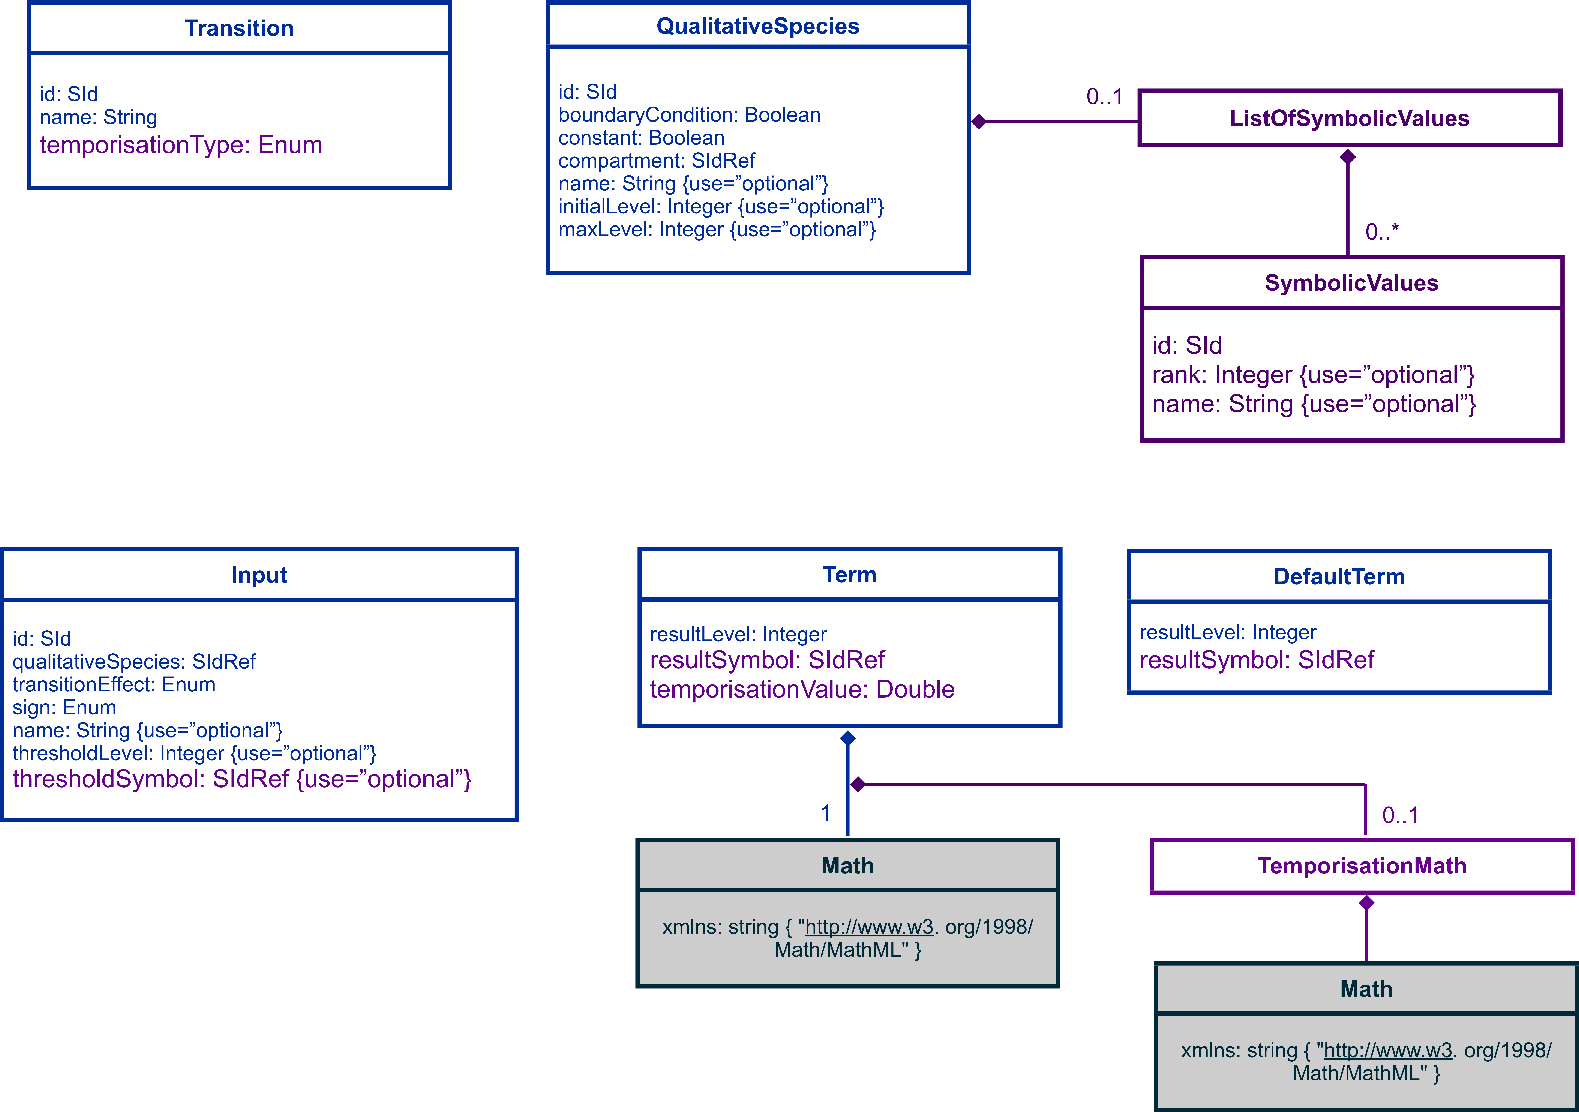
\includegraphics{figs/qual_future_directions.pdf}
%\caption {The definitions of the classe \listOf{SymbolicValues}, \qual{SymbolicValue} and \qual{TemporisationMath} and additional related attributes for existing classes.}
%  \label{qual_future_directions}
%\end{figure}


\subsection{Symbols}

\subsection*{Definition of \qualt{SymbolicValue}} % (fold)

\begin{figure}[hb]
  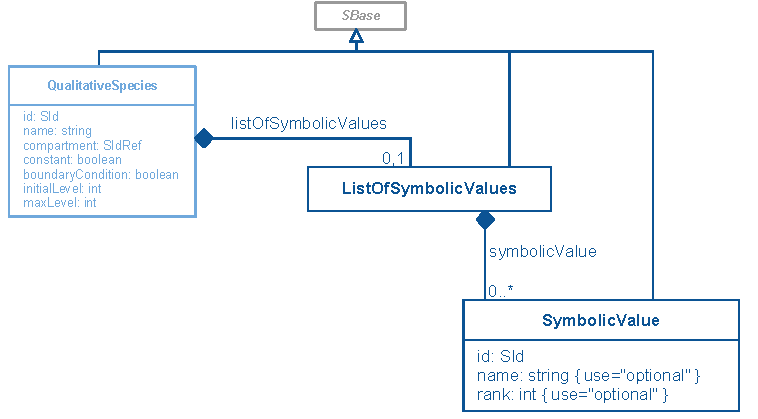
\includegraphics{figs/qual-qualitative-species-future-uml.pdf}
  \caption{Possible future extensions of the \QualitativeSpecies class.}
  \label{qual_future_directions}
\end{figure}

The \qual{QualitativeSpecies} element may contain at most one \listOf{SymbolicValues} that contains zero or more \qual{SymbolicValue}s. An empty list is allowed, and useful for e.g. adding annotations. 
The \qual{SymbolicValue} element defines a non instantiated parameter. Such symbols may represent the different solutions of piecewise linear differential equations, along with different thresholds.

\paragraph{The \attr{id} and \attr{name} attributes}
These attributes are used according to the SBML L3.1 Section 3.3. The attribute \attr{id} is mandatory and \attr{name} is optional. 

\paragraph{The \attr{rank} attribute}
The \attr{rank} is an \type{integer} that defines the position of the symbol in the \listOf{SymbolicValues}. This attribute is optional.


\paragraph{The \attr{thresholdLevel} and \attr{thresholdSymbol} attributes:} %% of Input
The \attr{thresholdLevel} is an \type{integer} and \attr{thresholdSymbol} is a \type{SIdRef}. They are optional and exclusive.

\paragraph{The \attr{resultLevel} and \attr{resultSymbol} attributes:} %% in FunctionTerm
The result of the term is described by a \attr{resultLevel} or a \attr{resultSymbol}. Both are optional, but one of them must be defined.


\const{assignmentSymbol}: The symbol associated to the \attr{qualitativeSpecies} is set to the \attr{resultSymbol} of the selected term.

\subsection{Temporisation}

\begin{figure}[hb]
  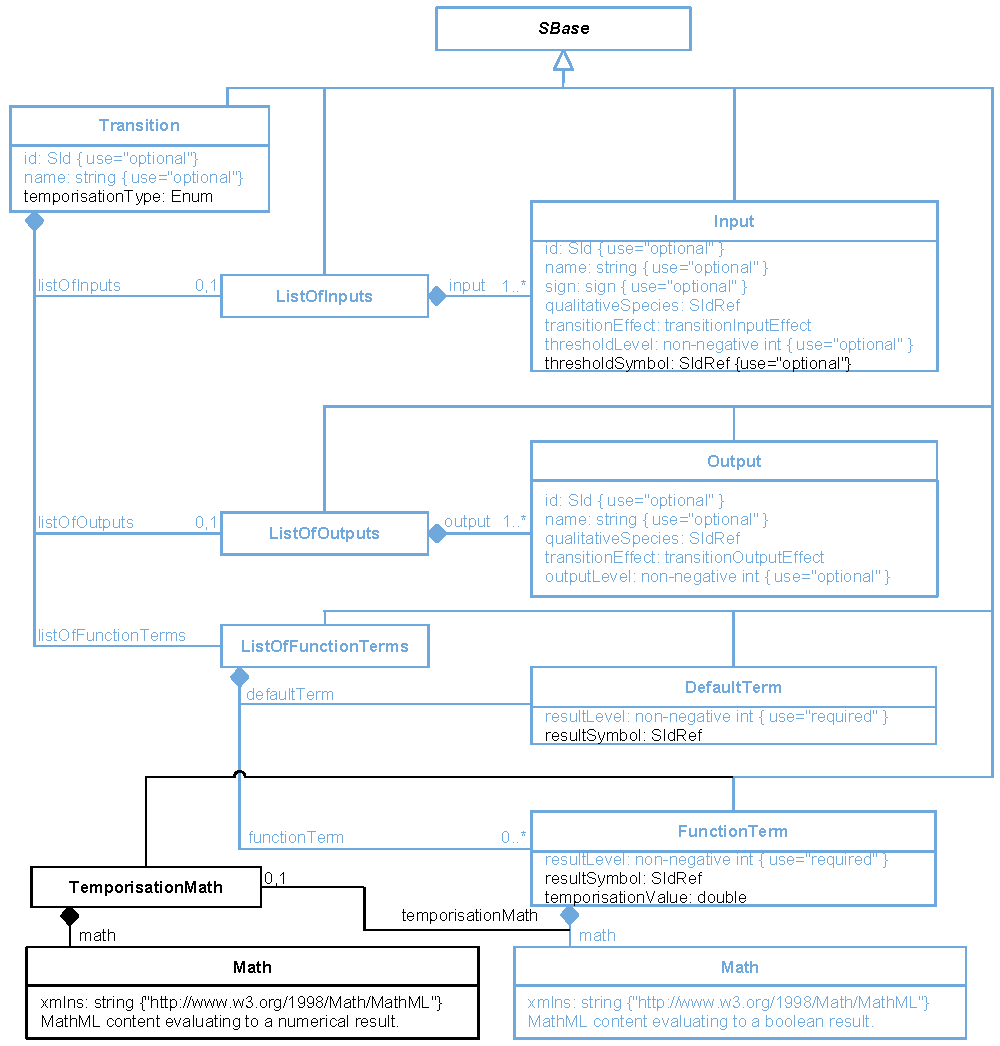
\includegraphics{figs/qual-transition-future-uml.pdf}
  \caption{Possible future extensions of the \Transition class.}
  \label{qual_future_directions}
\end{figure}

\paragraph{The \attr{temporisationType} attribute:} %% attribute of Transition
The \attr{temporisationType} is an \type{enumeration} the ``temporisation'' of the \qual{Transition}, that is the updating policy associated with the \qual{Transition}. It can be set to \const{timer}, \const{priority}, \const{sustain}, \const{proportion} or \const{rate}.
This attribute is optional. 



\paragraph{The \attr{temporisationValue} attribute and the \sbml{TemporisationMath} element:}
The attribute \attr{temporisationValue} and the element \sbml{TemporisationMath} allow the specification of the ``temporisation'' of the \qual{Transition} under the corresponding \qual{FunctionTerm}. Both are optional. Depending on the value of the \attr{temporisationType}, either one or both could be used.

The \attr{temporisationValue} is a \type{double}. The element \sbml{TemporisationMath} holds a MathML function returning a \type{double}. 

\hl{
\subsection{Classes of models and random models}}
\hl{
Several comments indicate that a future extension could support the representation of classes of models ({\it i.e.} models that are not fully parametrised, meaning that e.g. the logical rule of a component is incomplete), or random models, e.g. where several logical rules are associated to a component, the choice of a rule in the course of the dynamical evolution being arbitrary.
This might be done by revising the requirement of certain elements as well as the current semantics of {\em function terms}.}

\hl{\subsection{Interaction with SBML Core concepts}}
\hl{
At the time at which this Qualitative Modelling specification was developed, the policy and process for interacting with SBML Level 3 Core constructs was undefined. Thus, this particular specification does not facilitate the use of Core constructs. It is anticipated that in the future the specification will be extended to allow the use of these constructs; in particular Parameters and Events.
}

\subsection{Petri net models}

\textcolor{blue}{The current specification covers the needs of standard Petri Nets but provides a base for expansion to encompass more sophisticated modelling in this area. Both High Level Petri Nets (also referred to as Coloured PetriNets) and Timed PN should be achievable in future versions.}

\textcolor{blue}{We note that most PN models currently refer to metabolic or other reaction networks, and PN tools dedicated to this modelling framework often provides support for the SBML core format (see e.g. \cite{snoopy10}). }


